\chapter{Menginputkan File Excel Ke Dalam Database APEX}

\begin{enumerate}
\item[1]Buat Data akademik di excel dengan format .xlsx.

Pada data akademik ini terdapat 10 field yait npm, nama mahasiswa, alammat mahasiswa, tanggallahir, jurusan, kode matkul, nama matkul, indeks nilai, ruangan dan nama dosen.
    \begin{figure}[!htbp]
    \begin{center}
    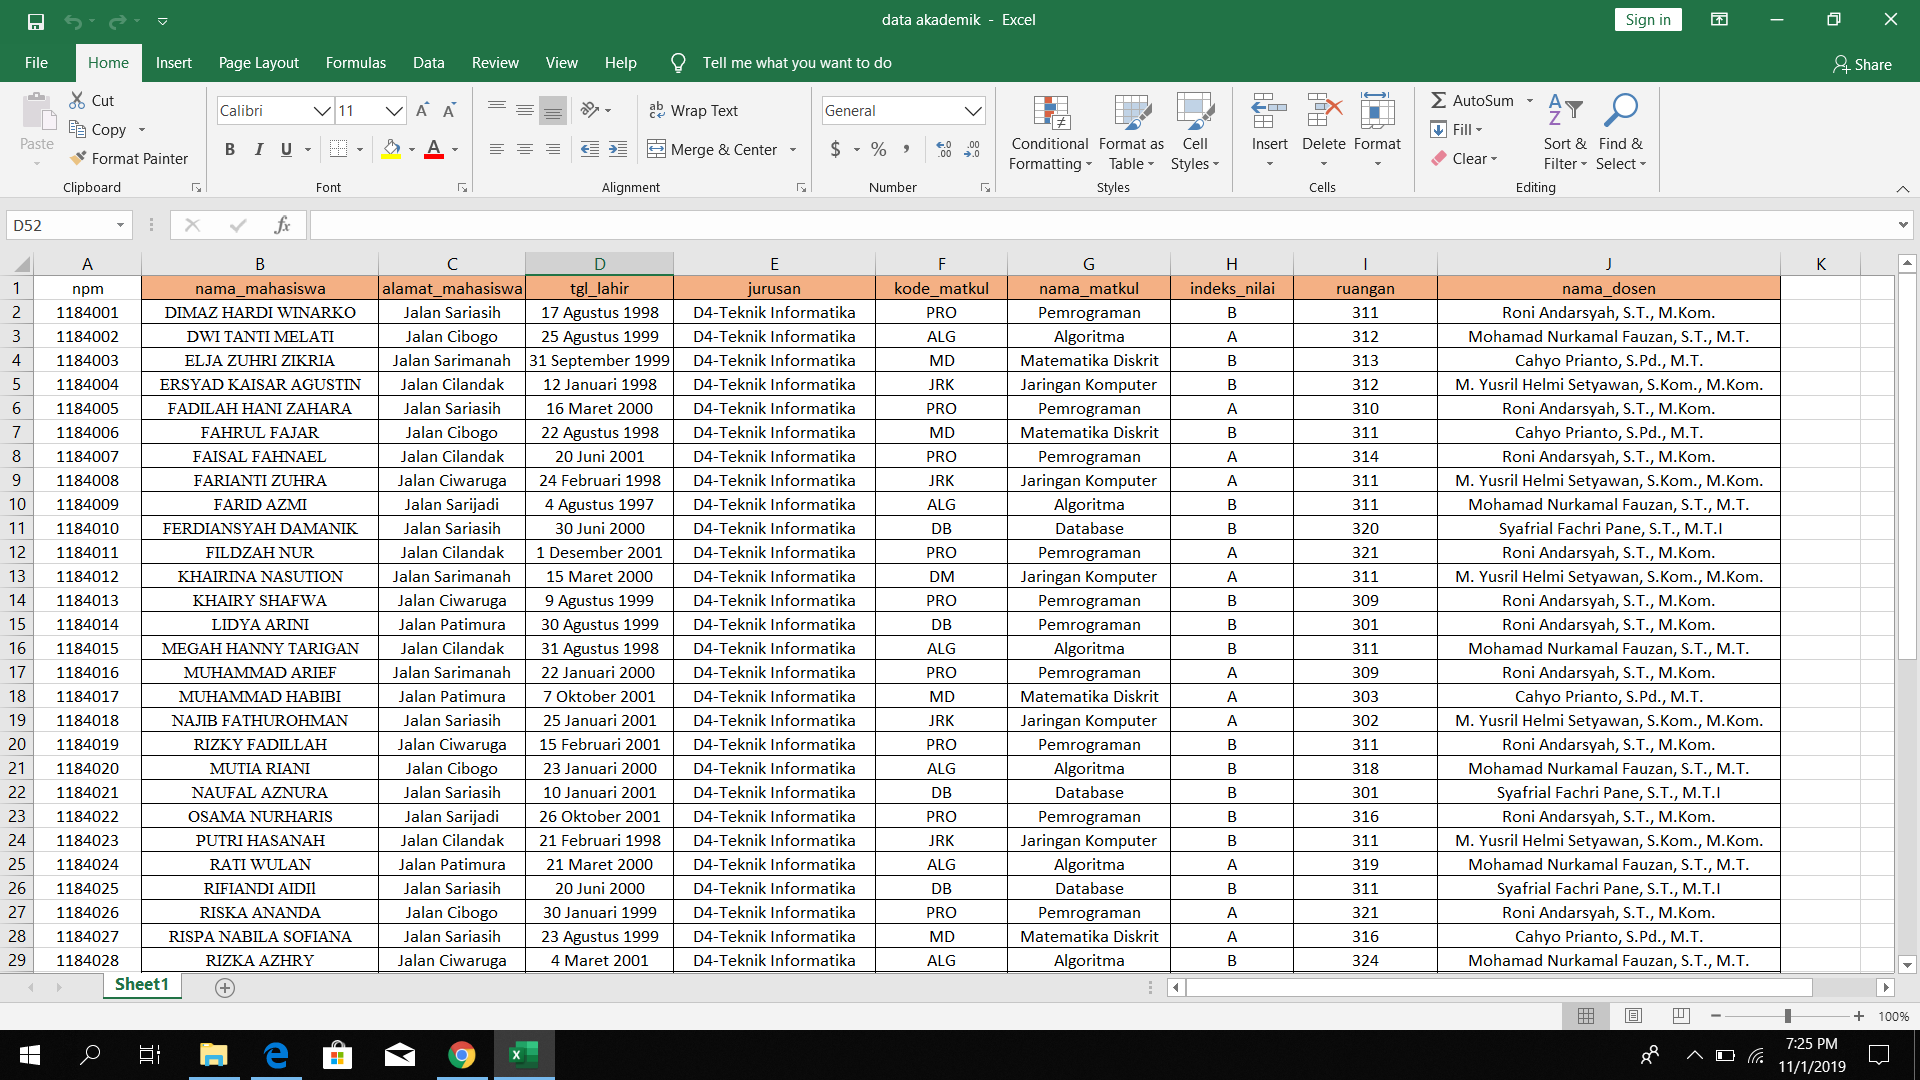
\includegraphics[scale=0.1]{figures/ss0.png}
    \caption{\textit{Contoh Isi File Tabel data Mahasiswa}}
    \end{center}   
\item[2]Masuk ke dalam Oracle APEX online Dan Workspace yang telah dibuat.

    \begin{center}
    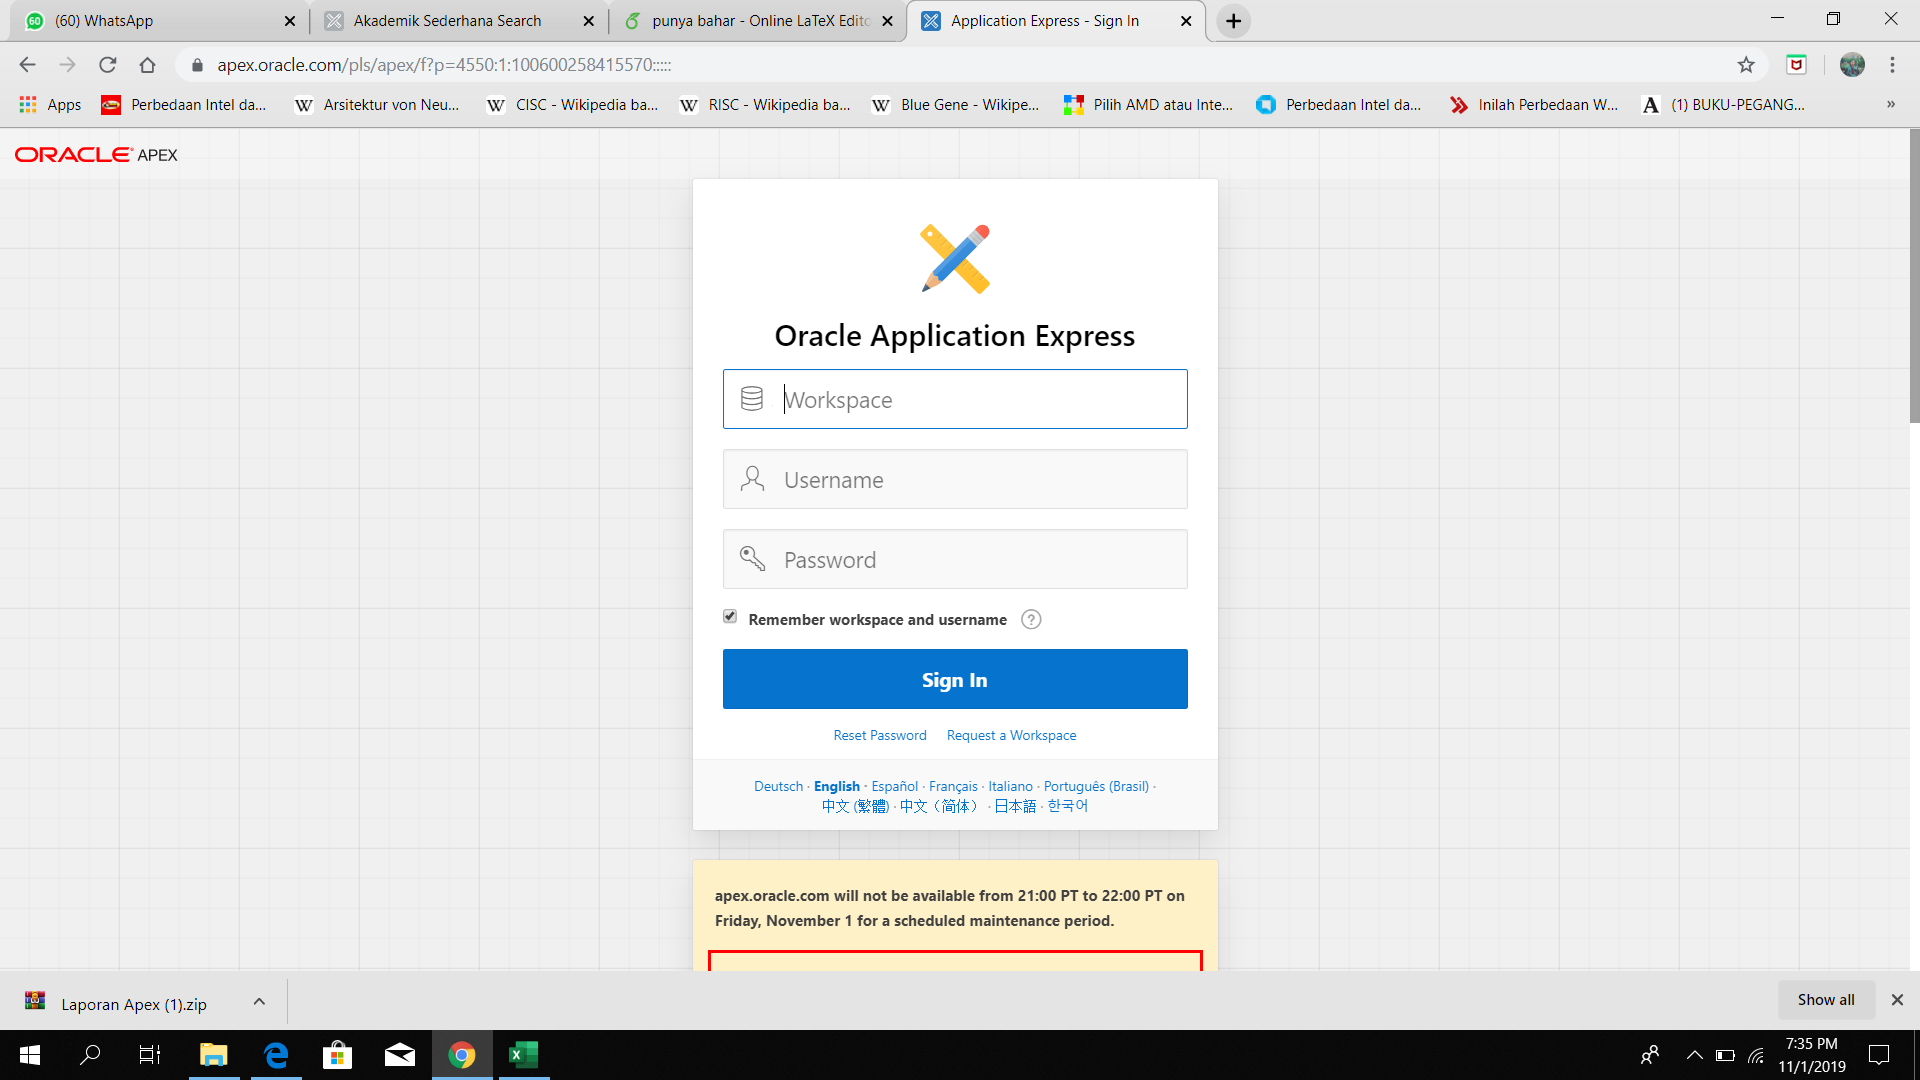
\includegraphics[scale=0.2]{figures/ss15.png}
    \caption{\textit{login.}}
    \end{center}
    \end{figure}
\begin{figure}[!htbp]
\item[3]setelah login, anda masuk ke halaman utama oracle apex online.

selanjutnya, anda pilih 'create' untuk membuat aplikasi database dari file excel.

    \begin{center}
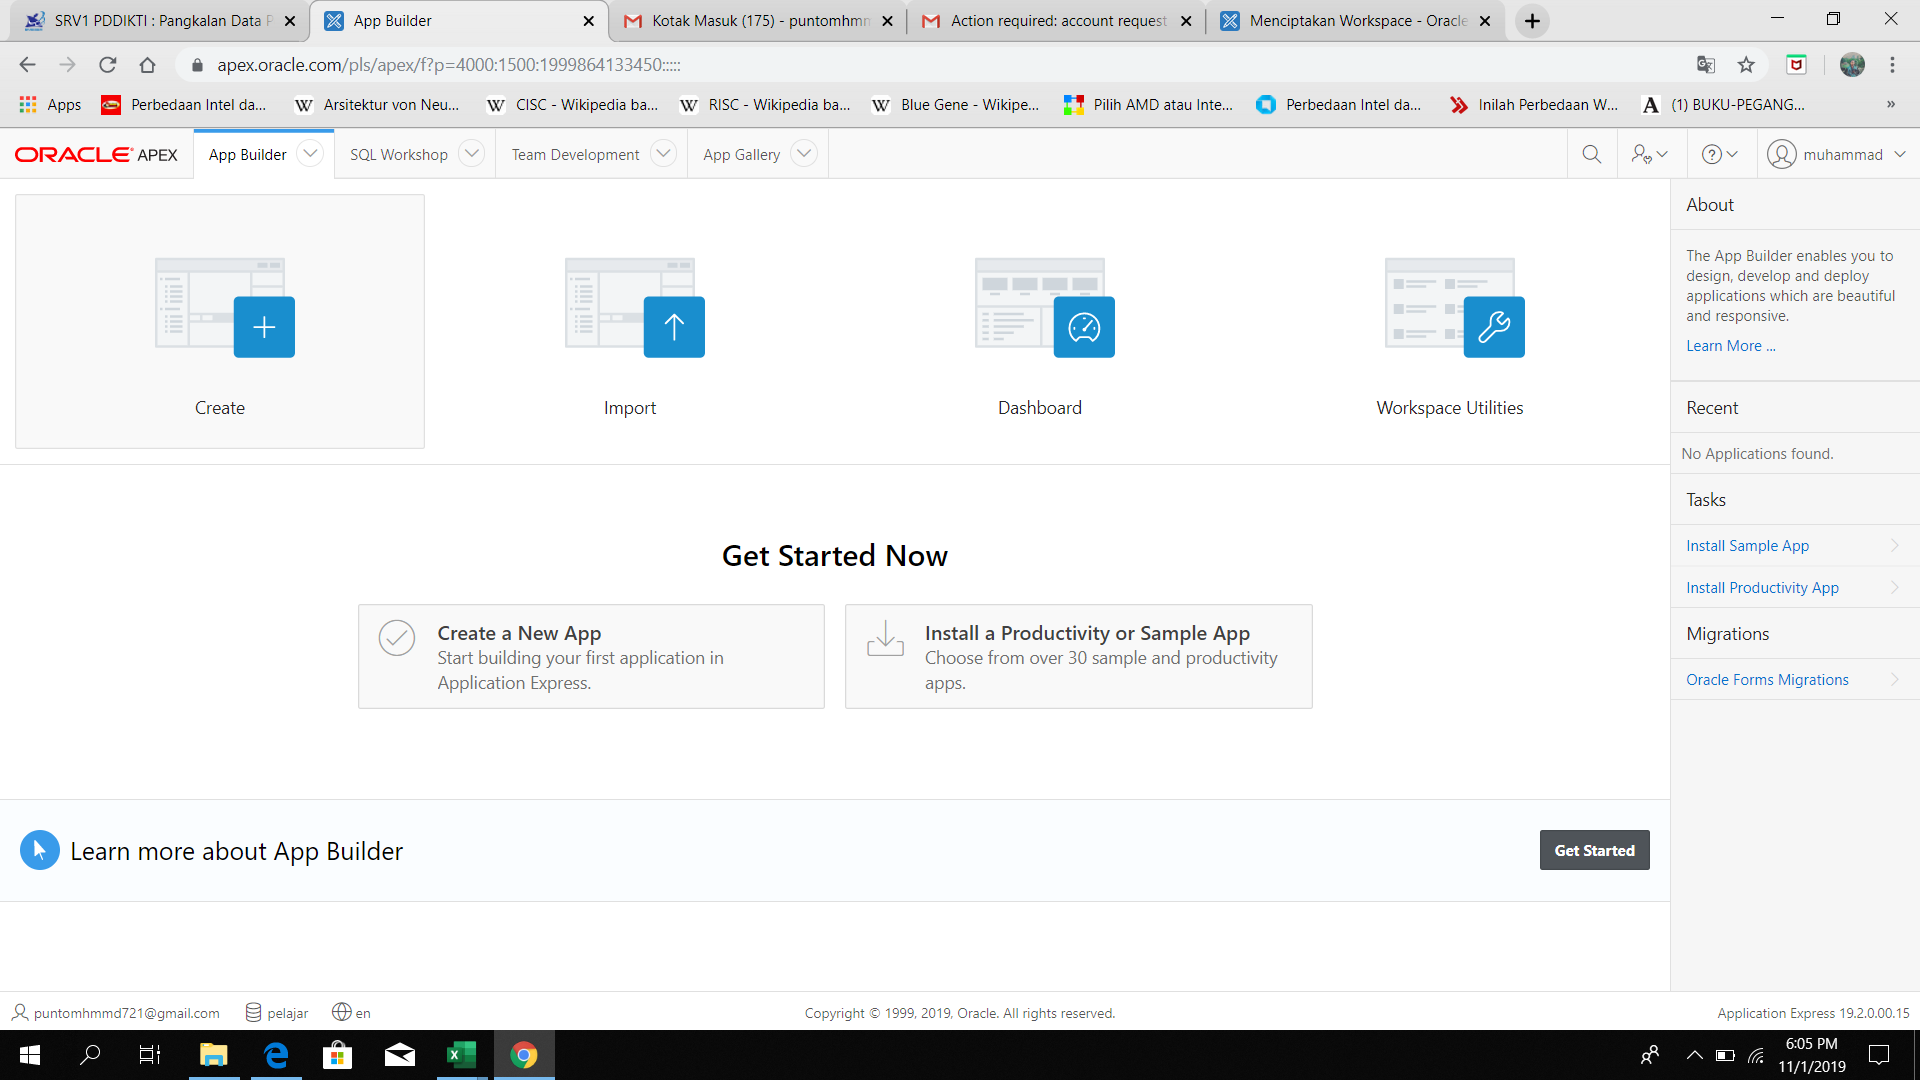
\includegraphics[scale=0.2]{figures/ss1.png}
    \caption{\textit{halaman utama apex online.}}
        \end{center}
        
\item[4]Pilih 'from a file' untuk mengupload file excel tersebut.  

    \begin{center}
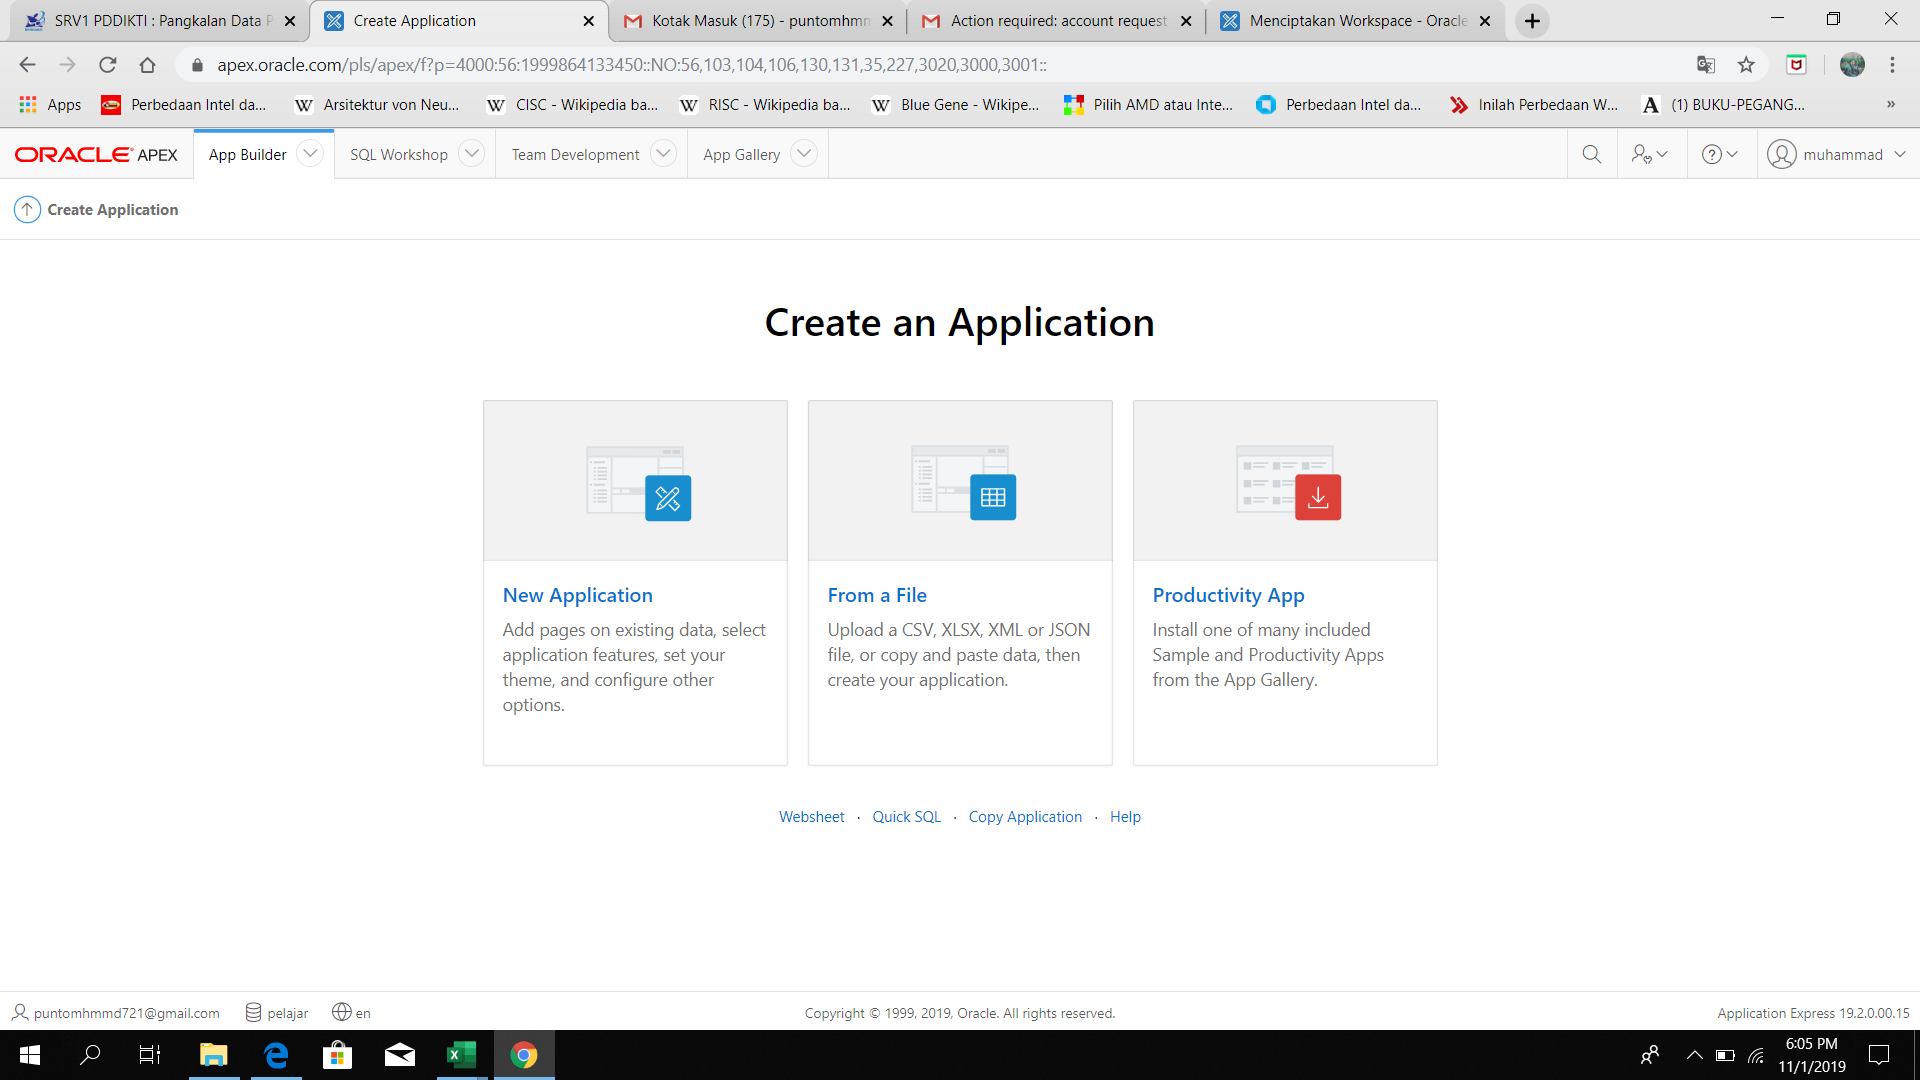
\includegraphics[scale=0.2]{figures/ss2.png}
    \caption{\textit{pilih 'from a file'}}
        \end{center}
        \end{figure}
\begin{figure}
\item[5]Masukkan file excel yang akan dijadikan aplikasi.

    \begin{center}
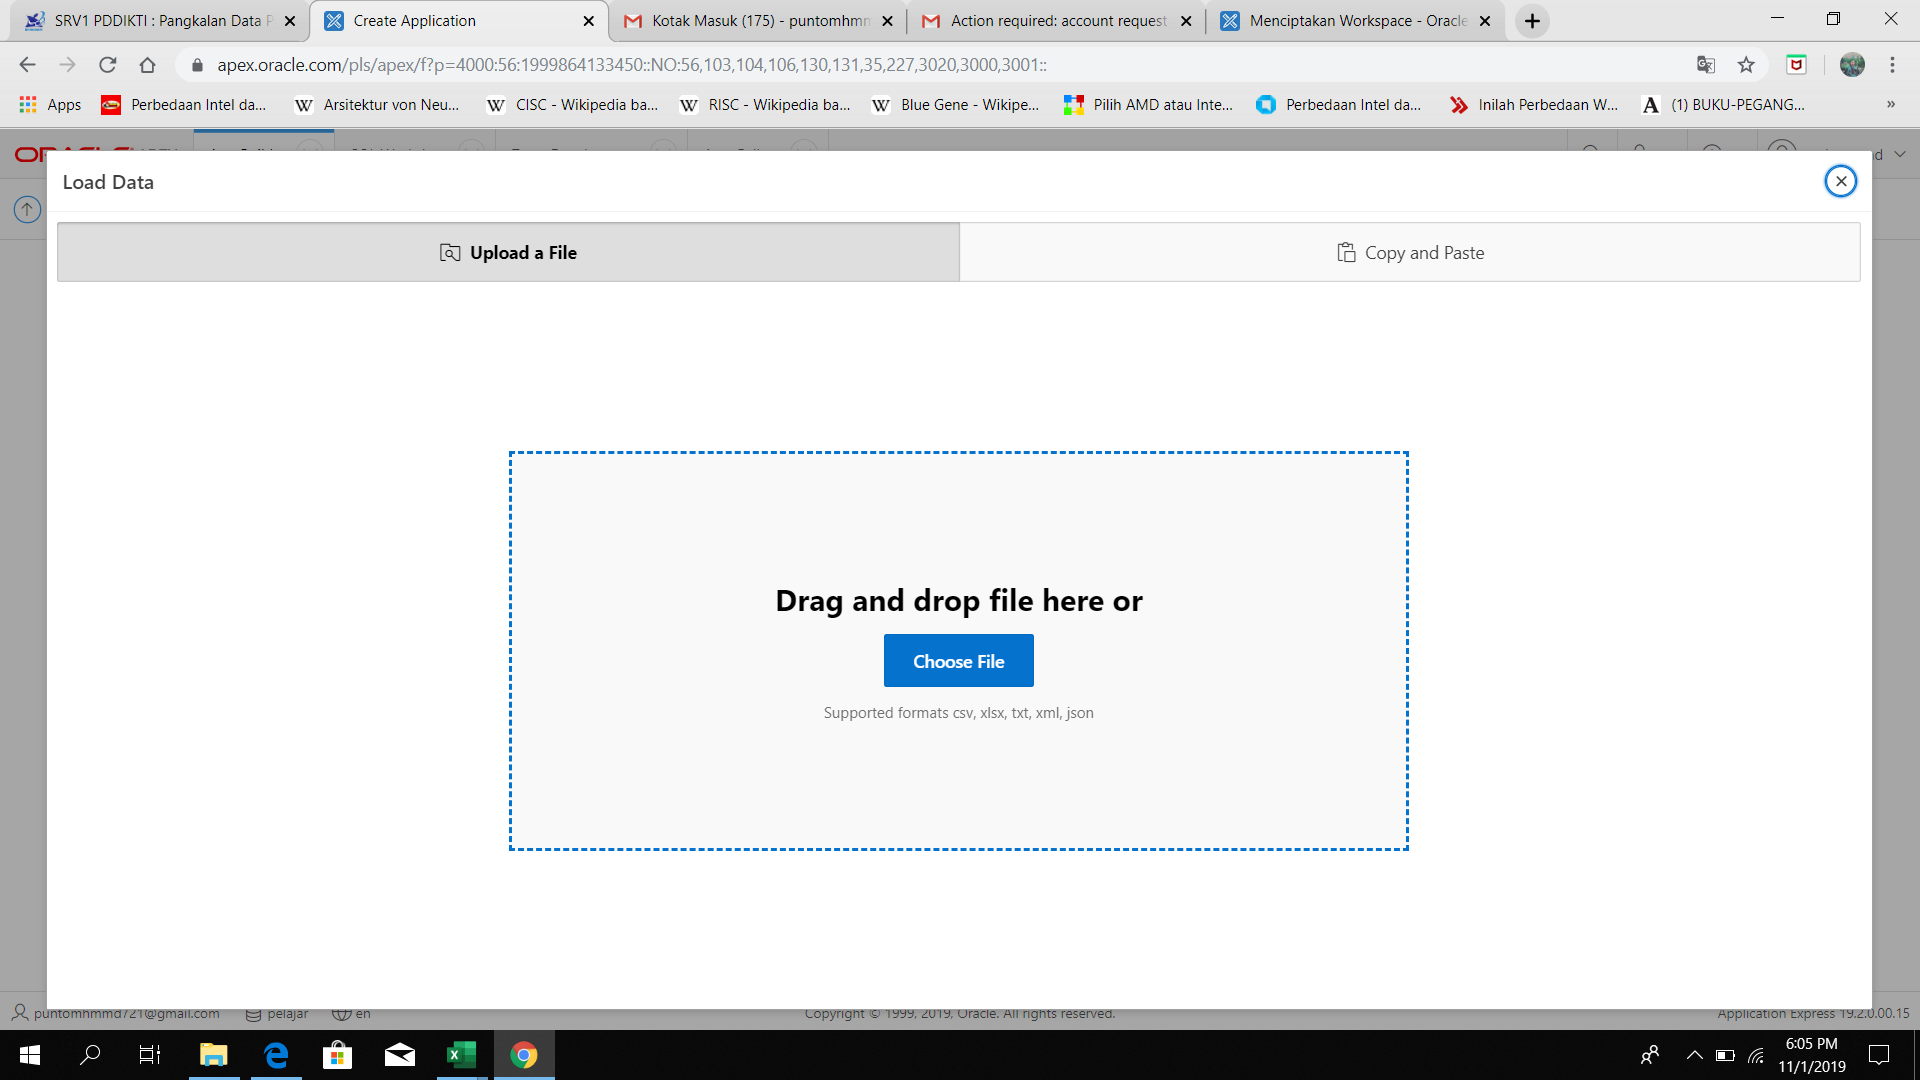
\includegraphics[scale=0.2]{figures/ss3.png}
    \caption{\textit{choose file.}}
        \end{center}

\label{gambar}
\end{figure}

\begin{figure}
\item[6] Anda masuk kde halaman load data.

pada halaman ini anda menginputkan 'table name' setelah itu pilih load data.

    \begin{center}
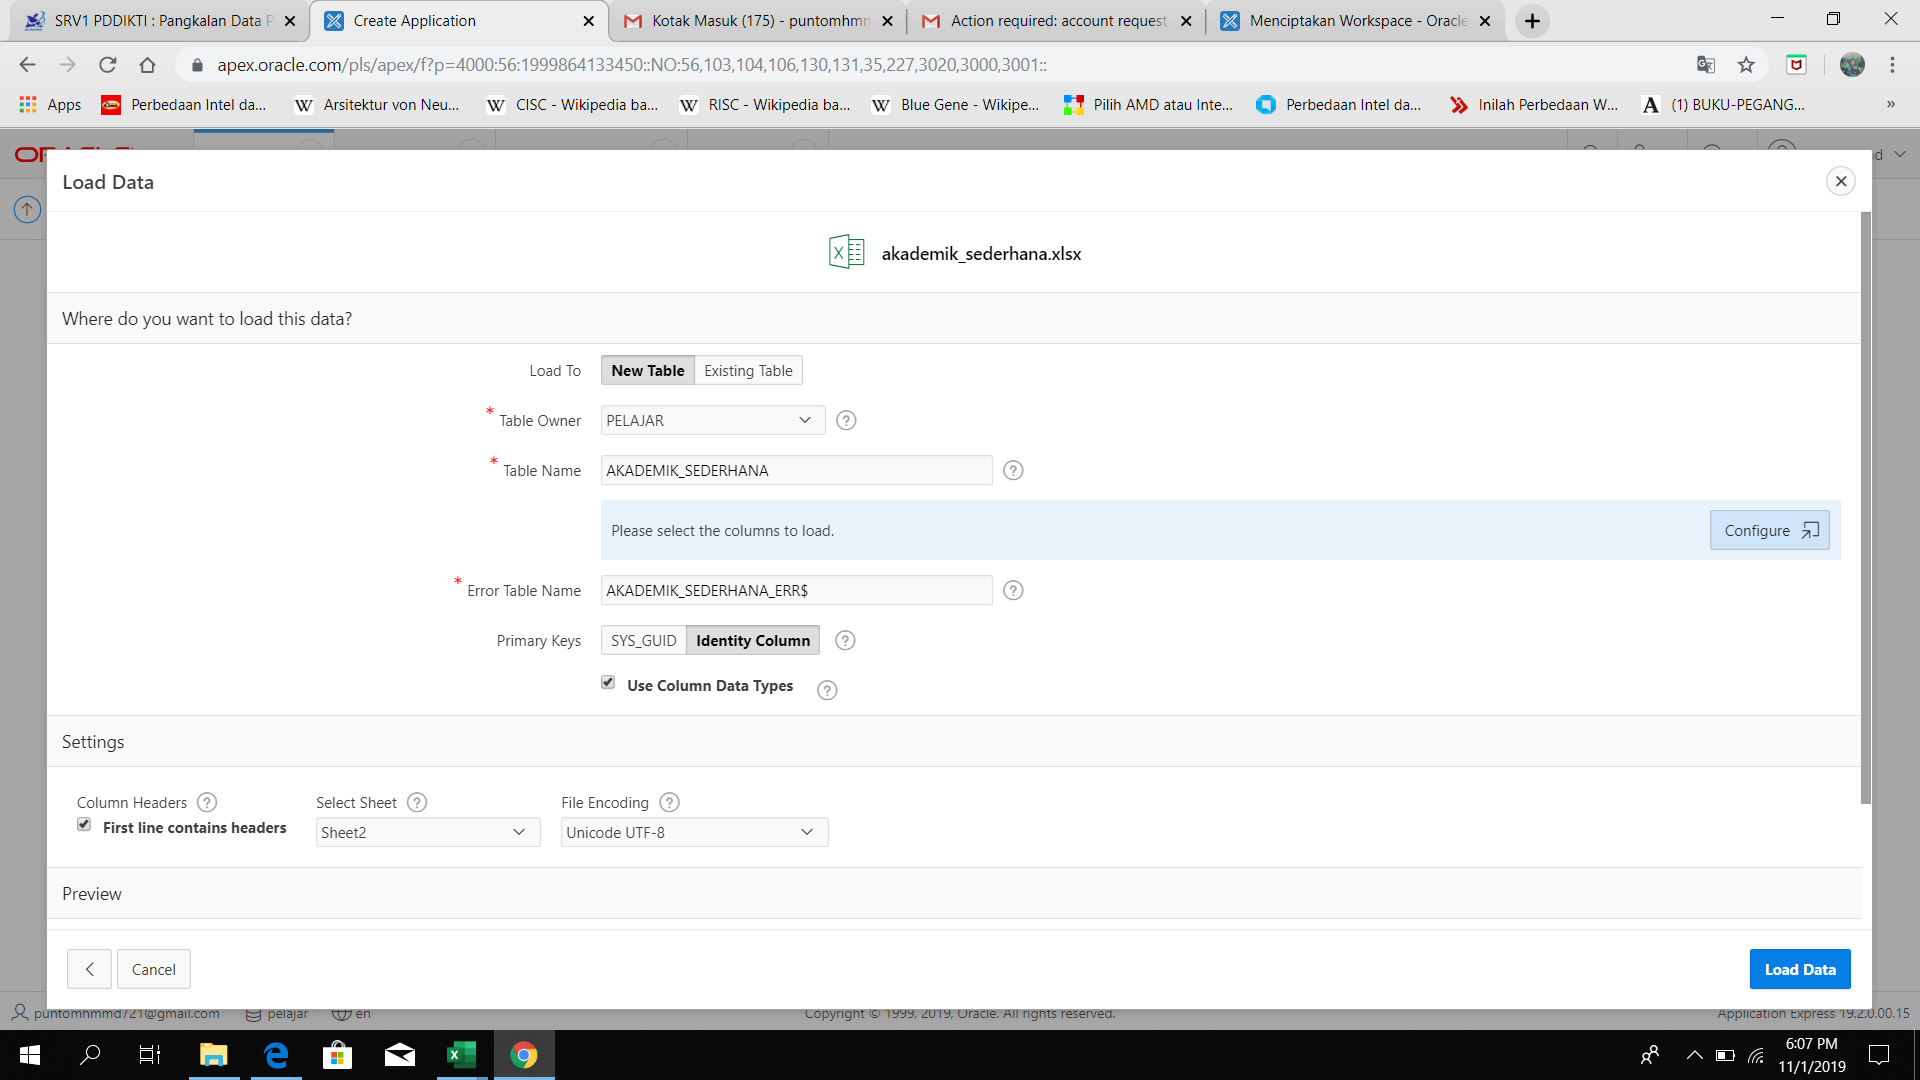
\includegraphics[scale=0.2]{figures/ss5.png}
    \caption{\textit{tampilan load data.}}
        \end{center}

\label{gambar}
\end{figure}

\begin{figure}
\item[7] selanjutnya akan dilaporkan kalau tabel telah dibuat.

    \begin{center}
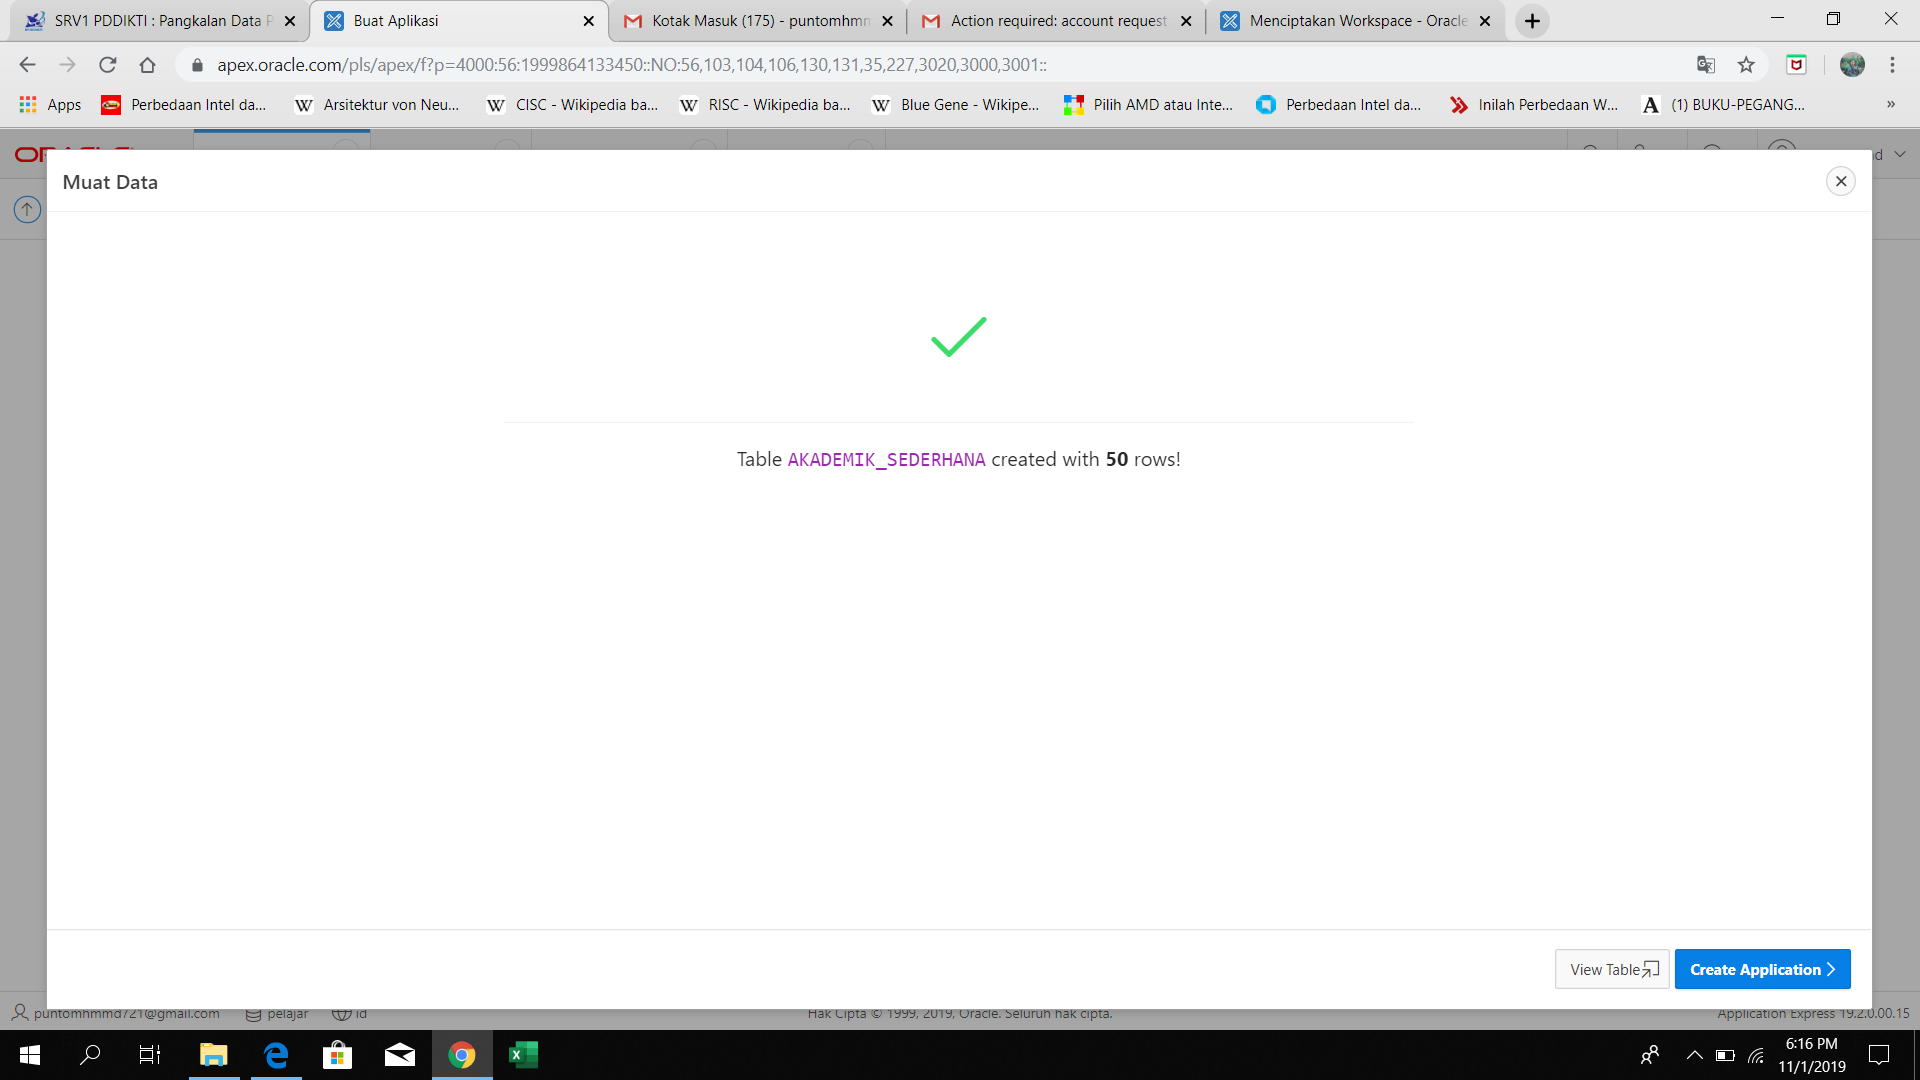
\includegraphics[scale=0.2]{figures/ss6.png}
    \caption{\textit{Konfirmasi tabel telah dibuat.}}
        \end{center}
\label{gambar}
\end{figure}

\begin{figure}
\item[8] Selanjutnya anda masuk ke halaman untuk membuat aplikasi akademik sederhana. setelah itu pilih 'creat aplication'.

    \begin{center}
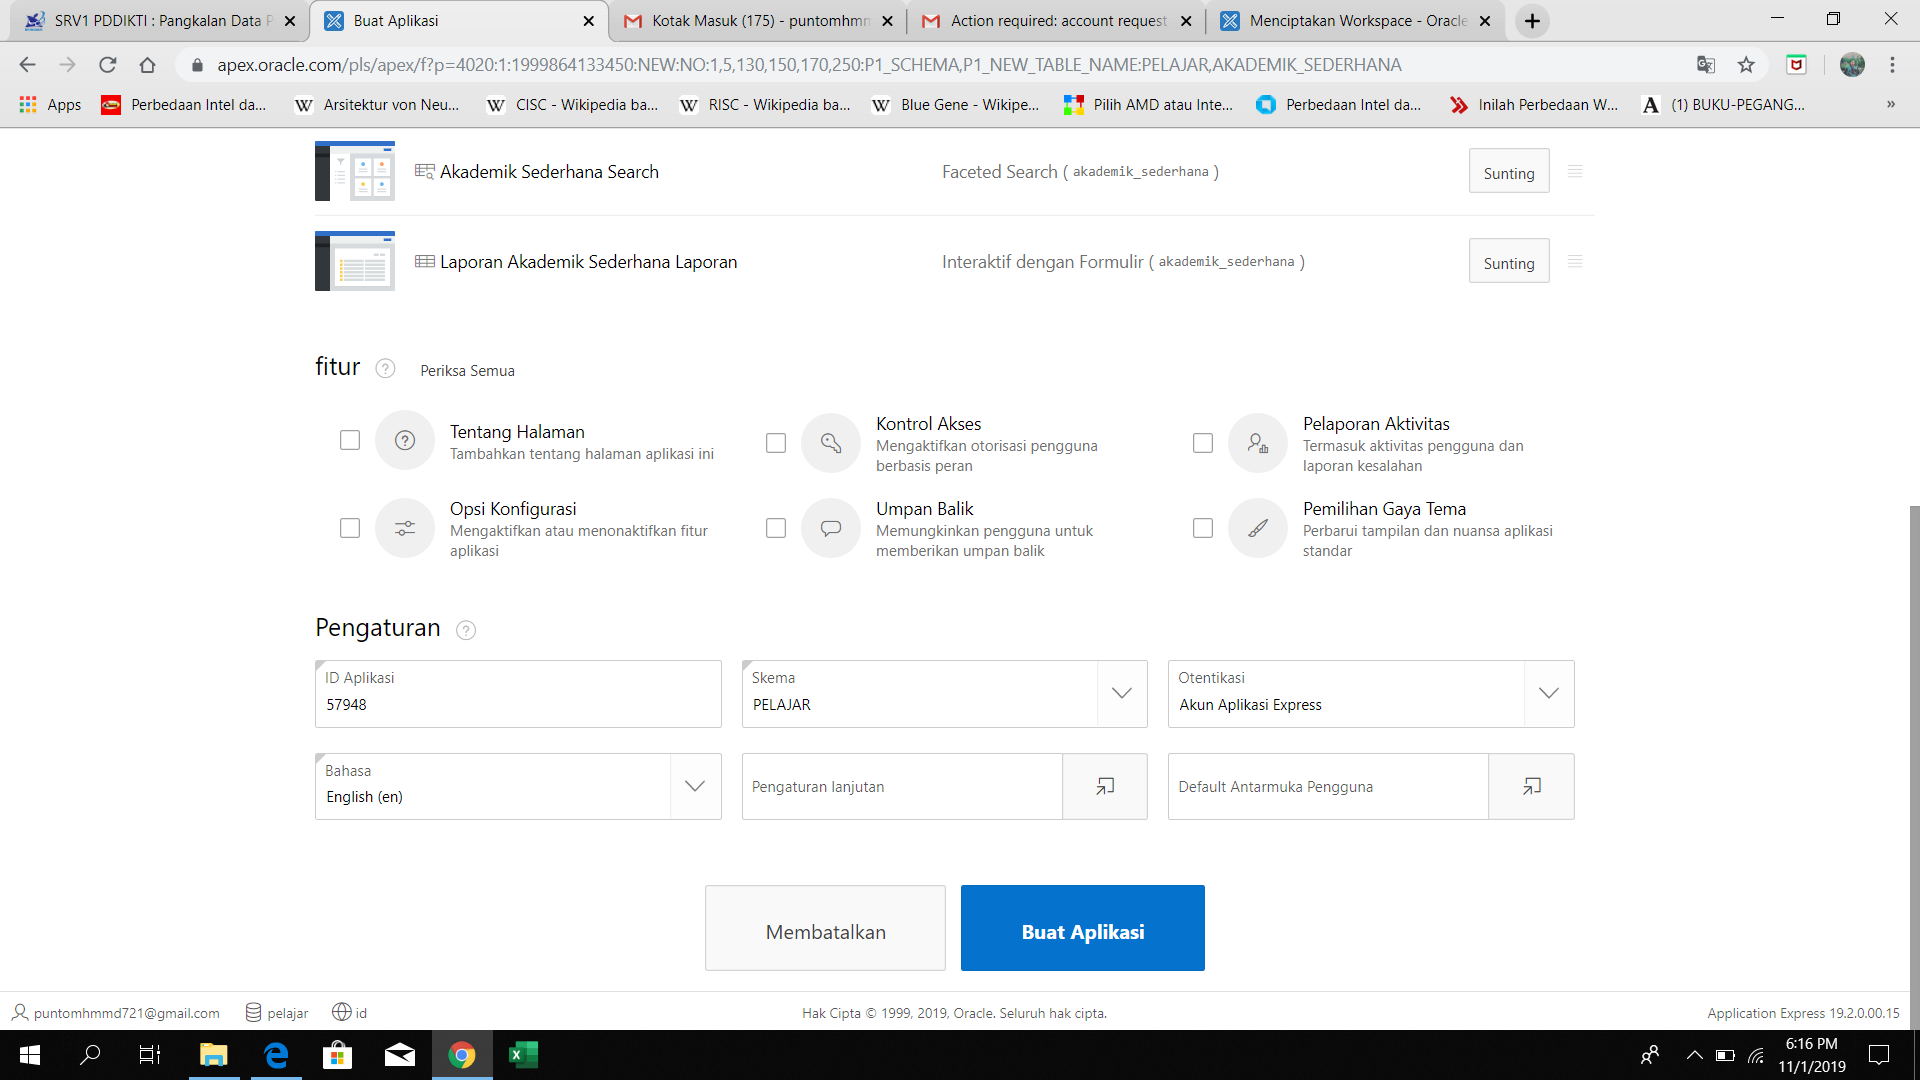
\includegraphics[scale=0.2]{figures/ss7.png}
    \caption{\textit{creat application.}}
        \end{center}
\label{gambar}
\end{figure}

\begin{figure}
\item[9] Setelah membuat application, anda dapat memilih 'run application' untuk menjalankan aplikasi.

    \begin{center}
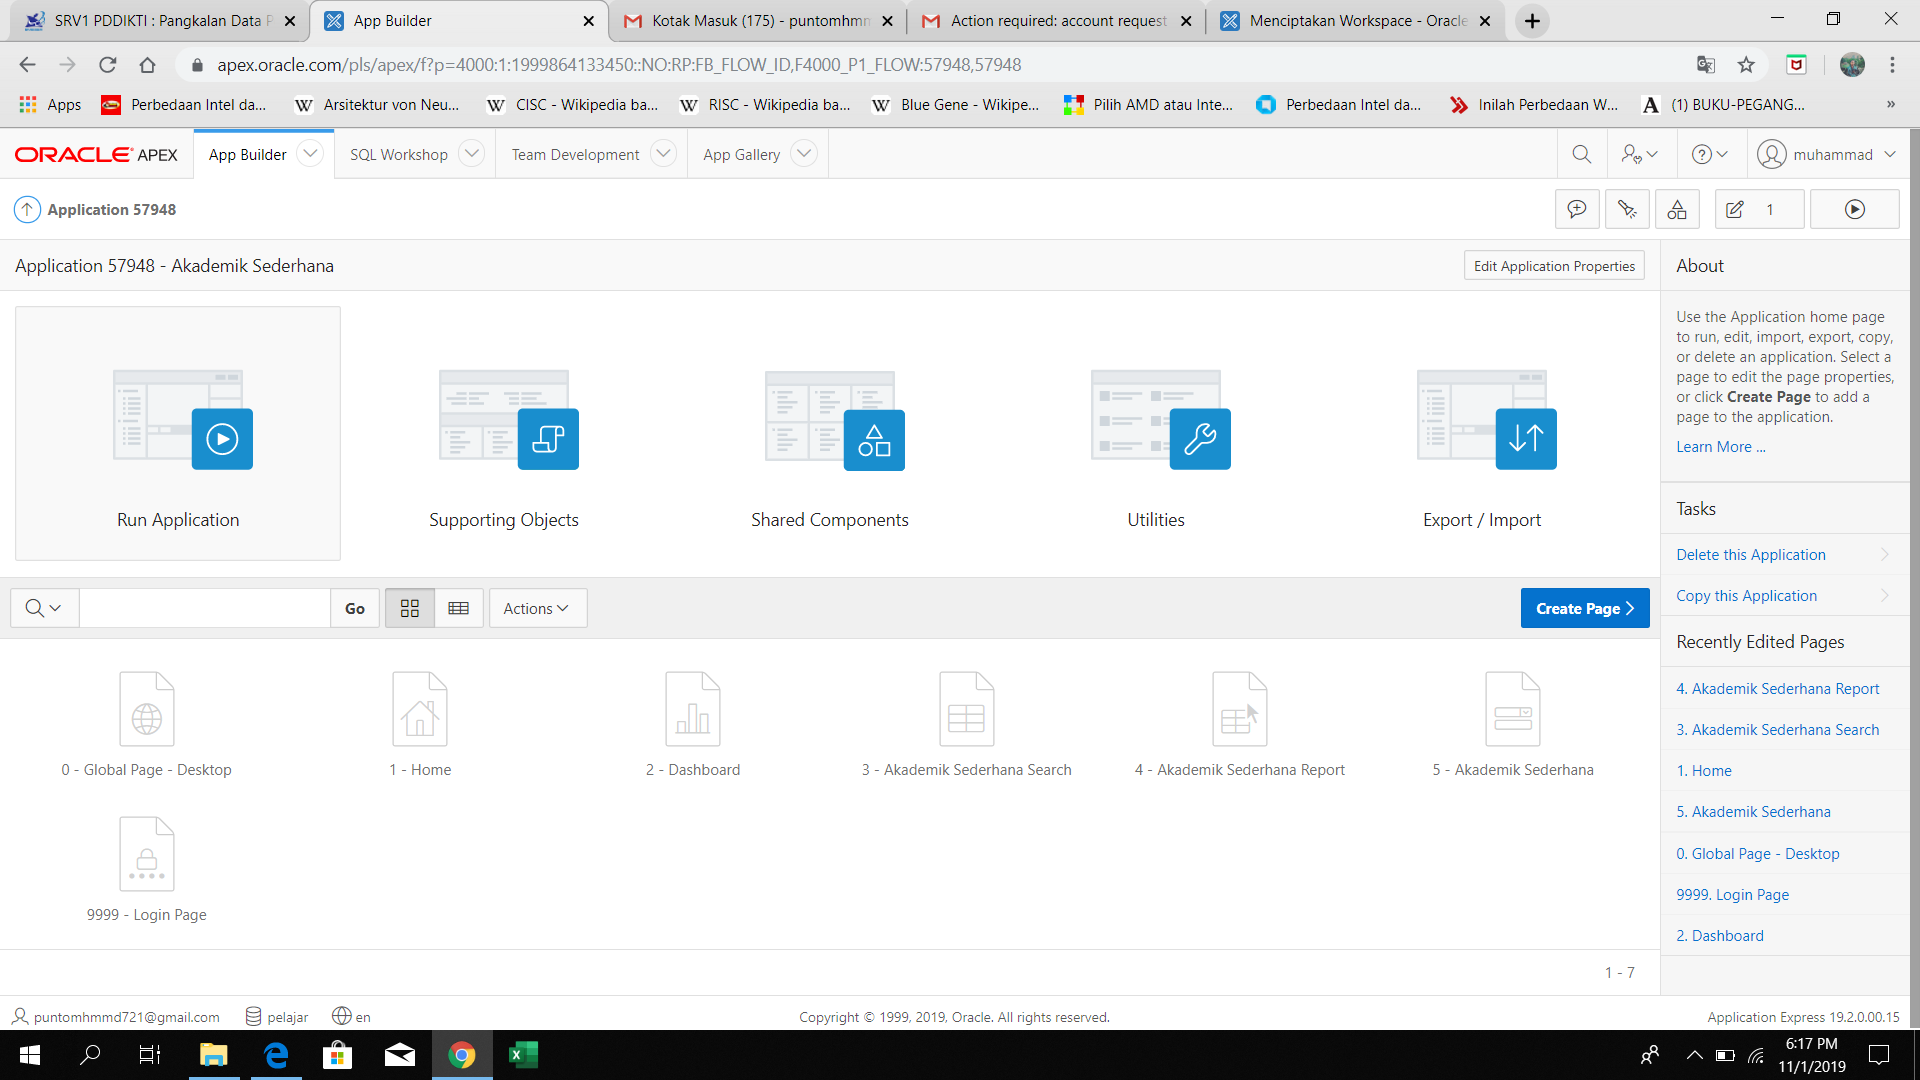
\includegraphics[scale=0.2]{figures/ss9.png}
    \caption{\textit{run application.}}
        \end{center}
\label{gambar}
\end{figure}

\begin{figure}
\item[10] selanjutnya anda login ke dalam aplikasi akademik sederhana yang telah dibuat menggunakan username dan password anda sebelumnya.


aplikasi: https://apex.oracle.com/pls/apex/f?p=58606:3:30755701303895::NO:::


username : puntomhmmd097@gmail.com


password : bismillah721

    \begin{center}
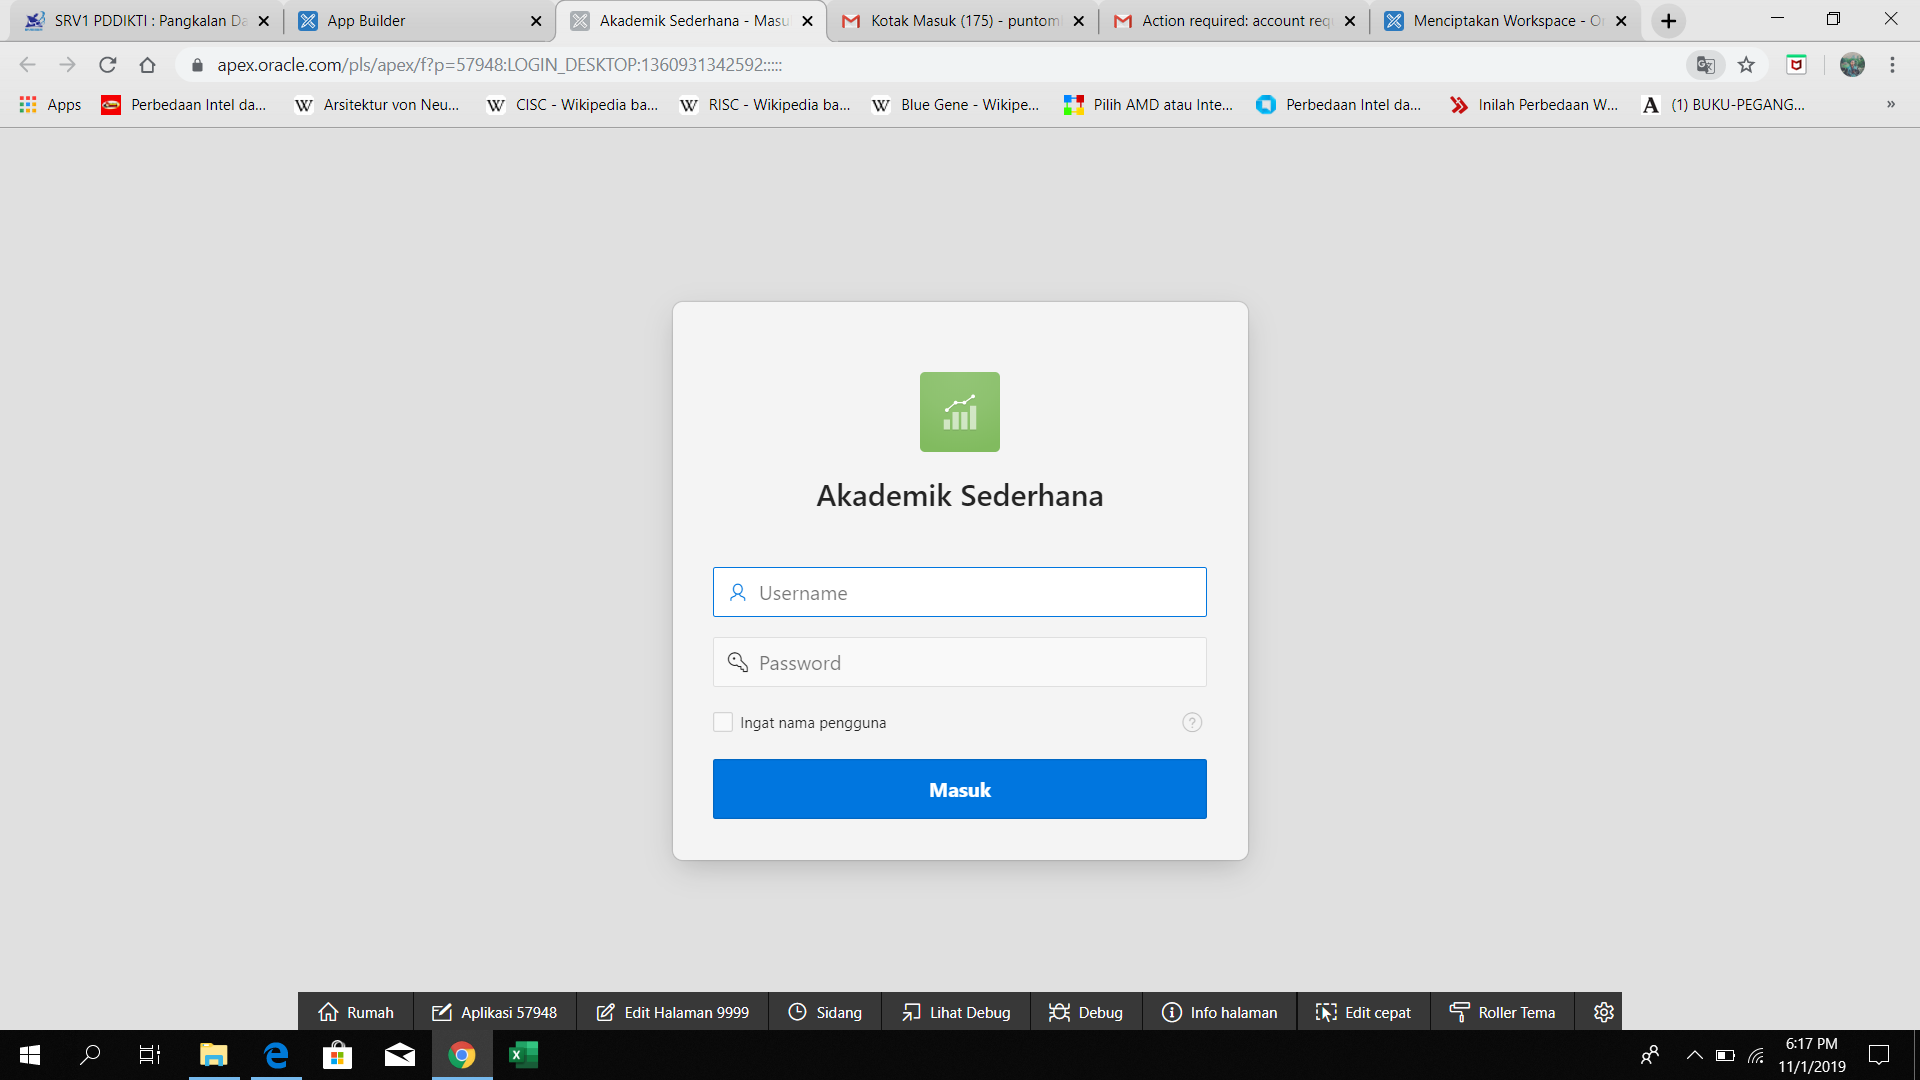
\includegraphics[scale=0.2]{figures/ss10.png}
    \caption{\textit{Login ke aplikasi.}}
        \end{center}
\label{gambar}
\end{figure}

\begin{figure}
\item[11] Masuk kedalam halaman home aplikasi Akademik Sederhana yang telah dibuat.

    \begin{center}
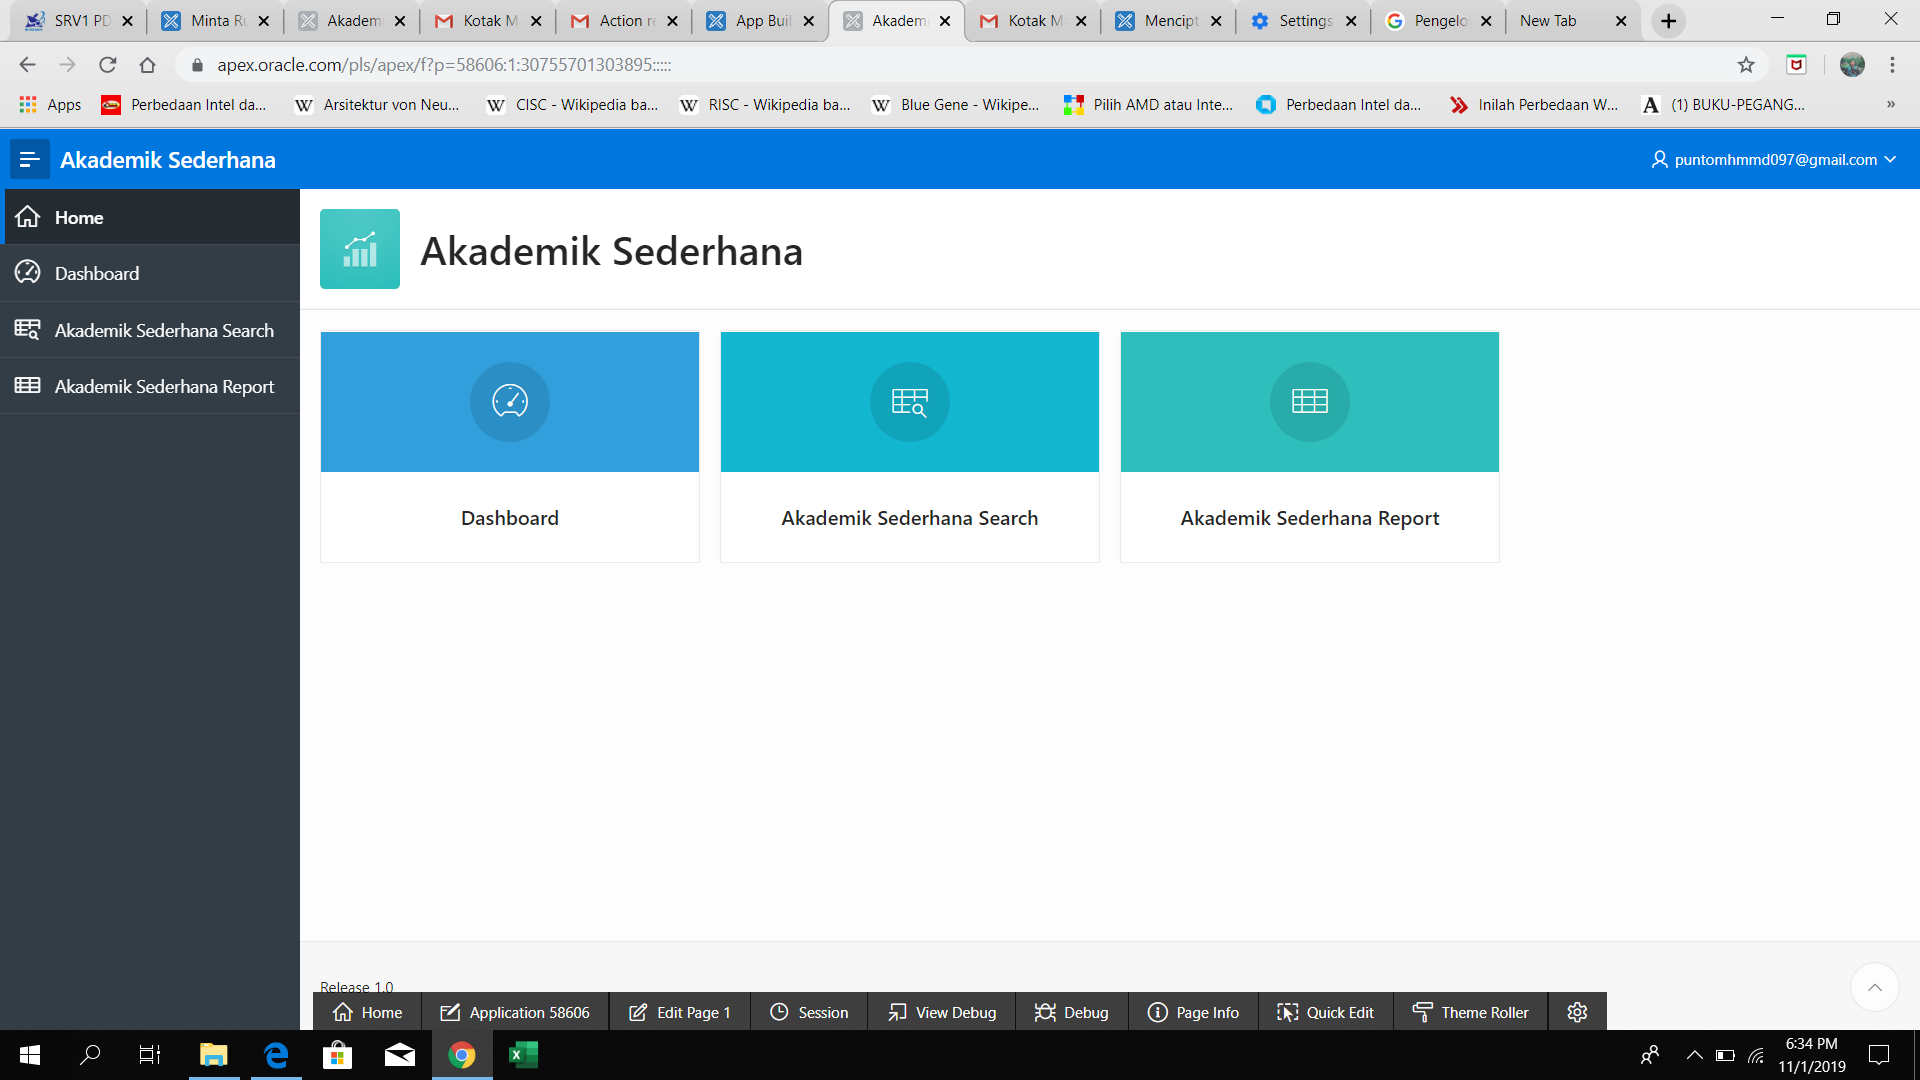
\includegraphics[scale=0.2]{figures/ss11.png}
    \caption{\textit{Tampilan Home.}}
        \end{center}
\label{gambar}
\end{figure}

\begin{figure}
\item[12] Halaman Dashboard aplikasi Akademik Sederhana.

    \begin{center}
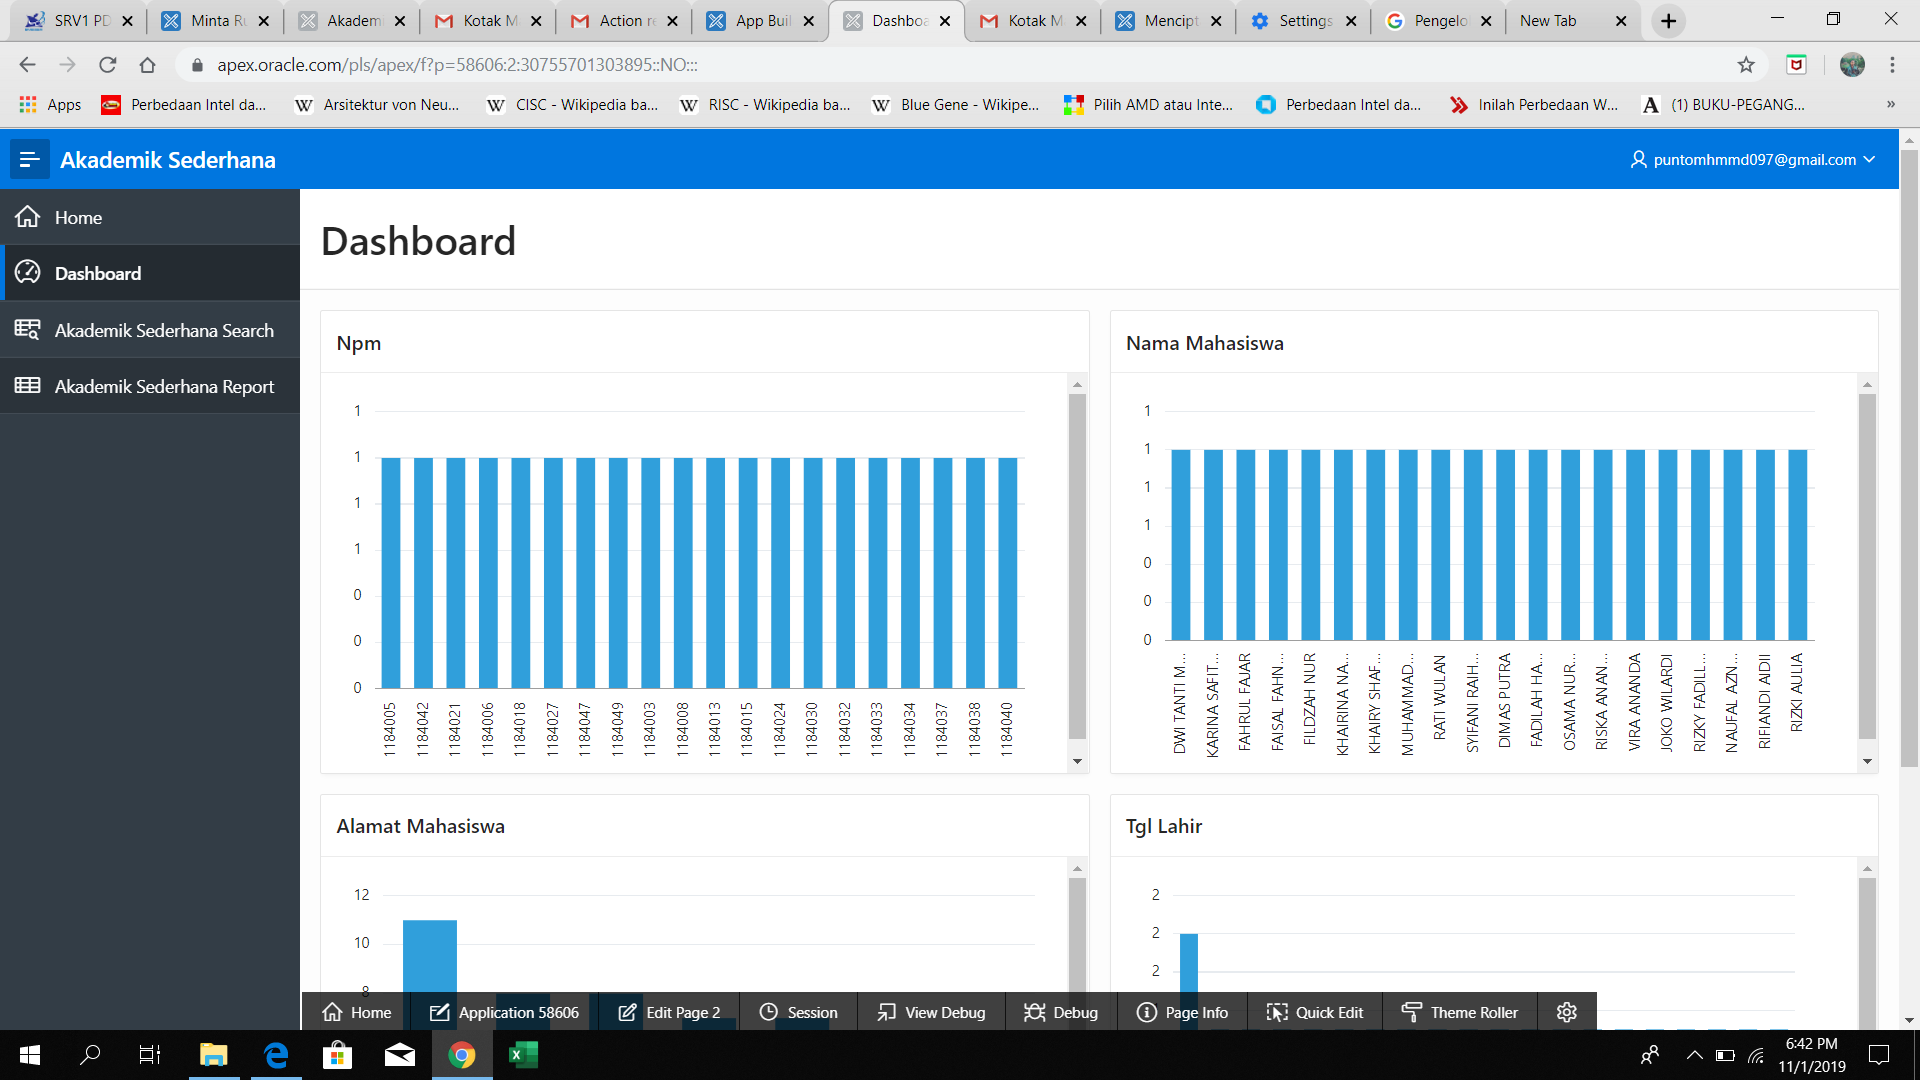
\includegraphics[scale=0.2]{figures/ss12.png}
    \caption{\textit{Tampilan Halaman DashBoard.}}
        \end{center}
\label{gambar}
\end{figure}

\begin{figure}
\item[13] Tampilan halaman akademik sederhana search.

    \begin{center}
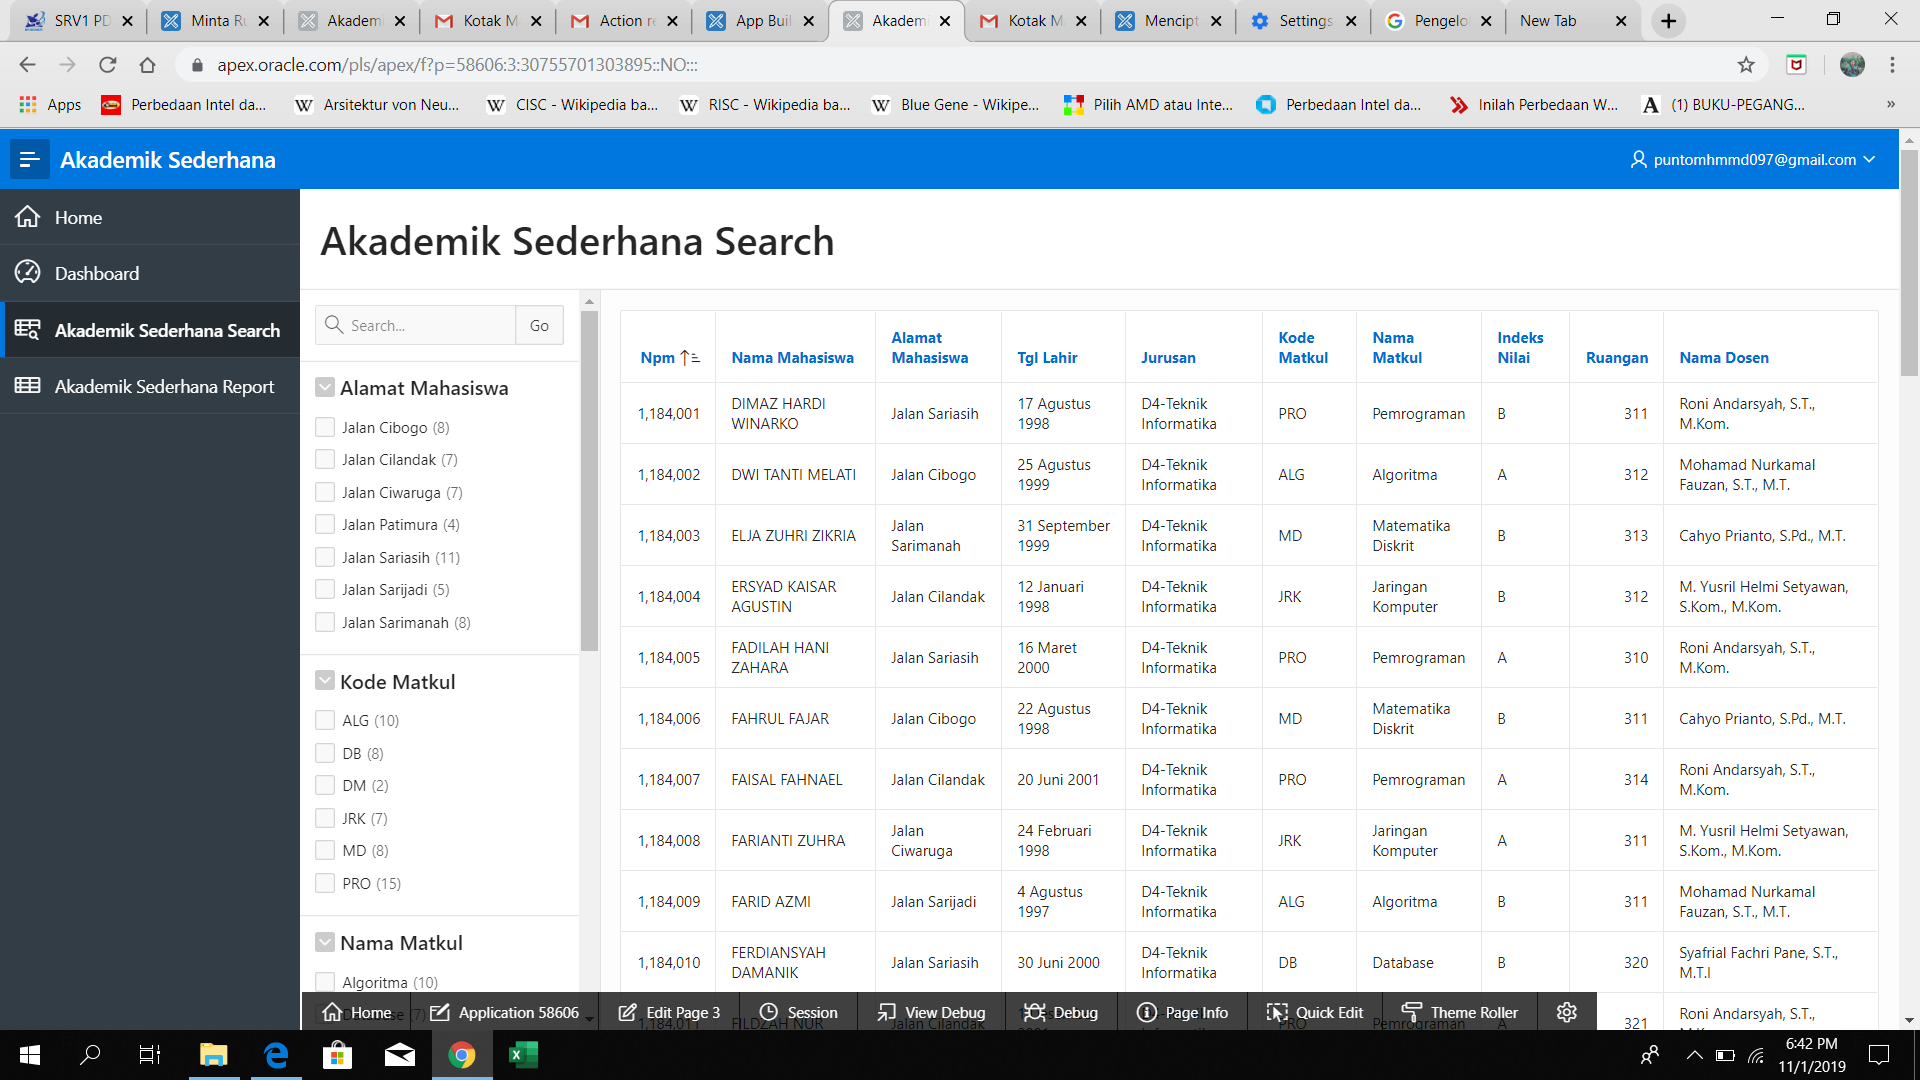
\includegraphics[scale=0.2]{figures/ss13.png}
    \caption{\textit{Tampilan Halaman Akademik Sederhana Search}}
        \end{center}
\label{gambar}
\end{figure}

\begin{figure}
\item[14] Tampilan halaman akademik sederhana report.

    \begin{center}
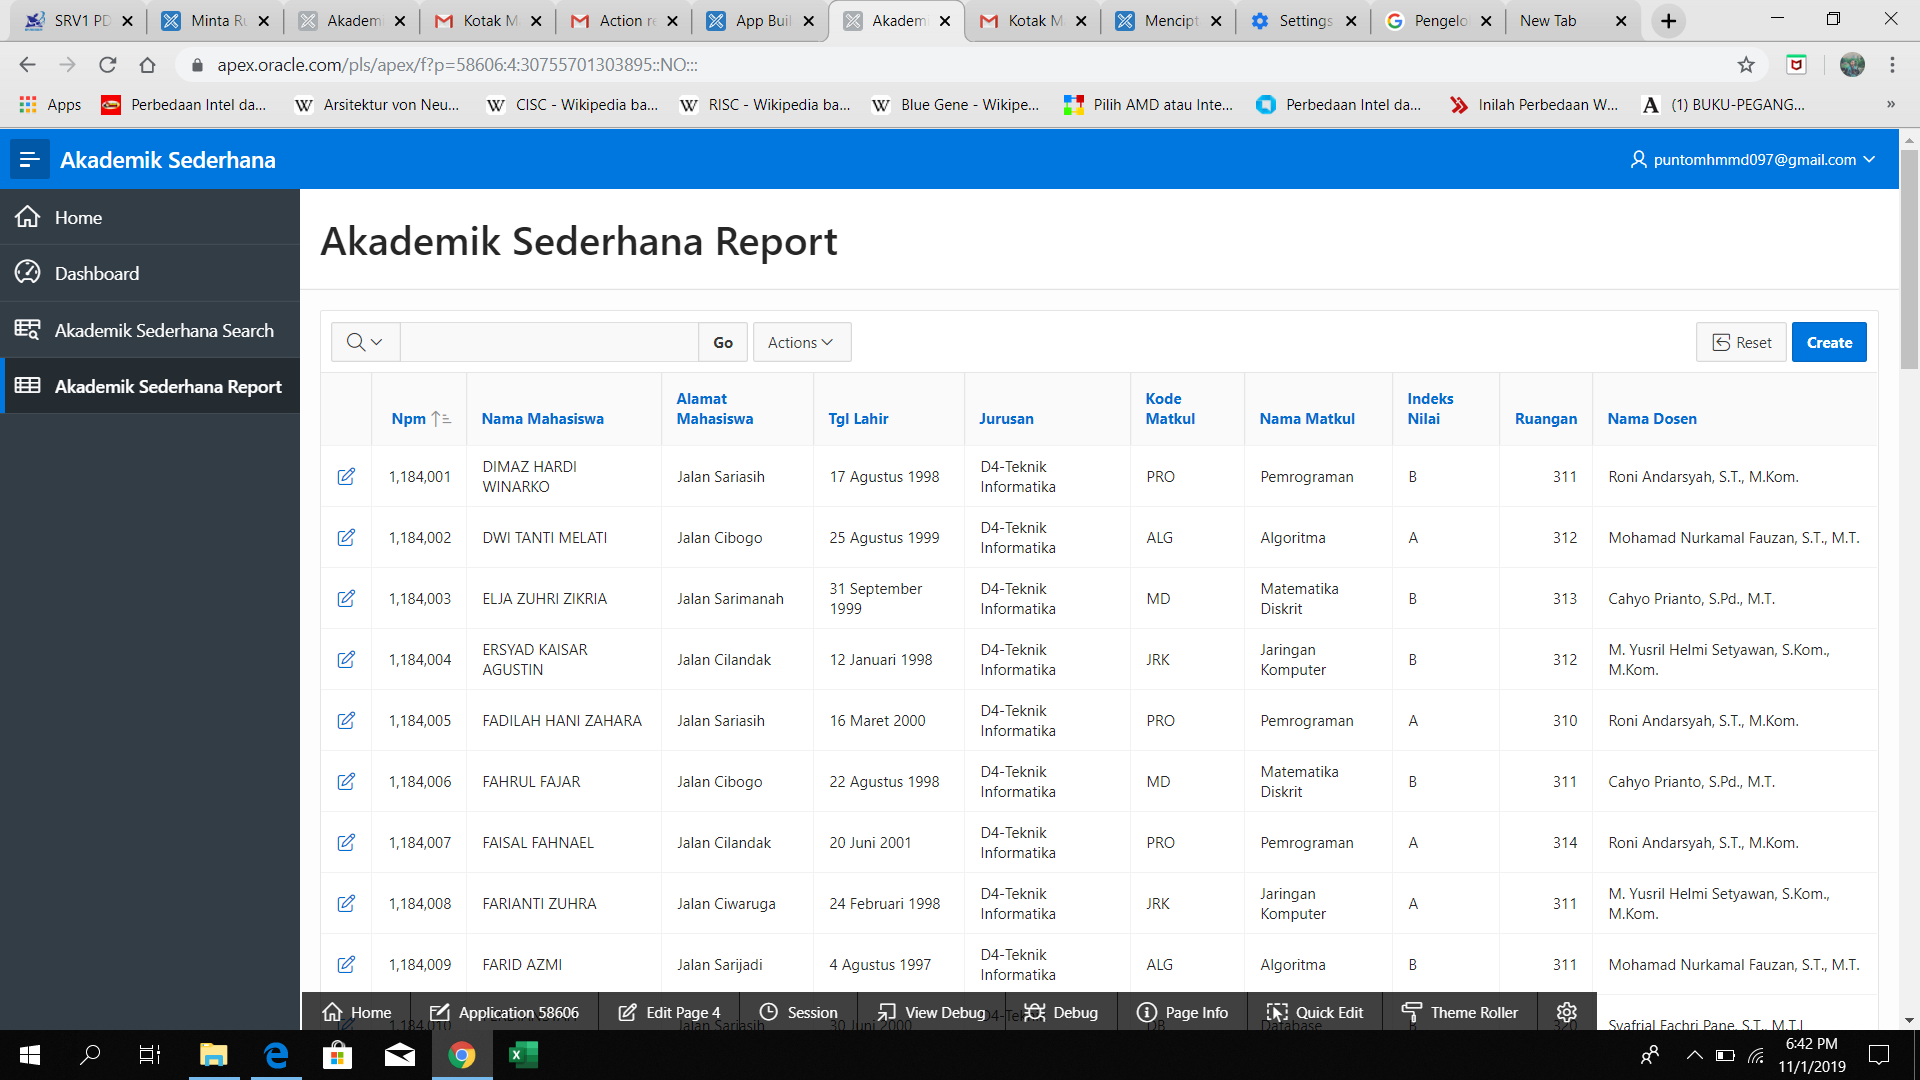
\includegraphics[scale=0.2]{figures/ss14.png}
    \caption{\textit{Tampilan Halaman Akademik Sederhana.}}
        \end{center}
\label{gambar}
\end{figure}

\end{enumerate}
